\section {Exploring Thread Interleaving Space}
\label{s:design}

In this section, we describe our approach to effectively achieve
\textbf{Design goal 1} and \textbf{2}.
%
We first explain the key idea of our approach~(\autoref{ss:overview}).
Then, we illustrate our concurrency coverage metric to express
combinatorial interleavings (\textbf{Design goal
  1})~(\autoref{ss:coverage}), and the interleaving search strategy to
cleverly explore thread interleavings (\textbf{Design goal
  2})~(\autoref{ss:scheduler}).
%While this section focuses only on how to explore the search space of
%thread interleaving with a given multi-thread input, the whole design
%of \sys will be explained later in \autoref{s:impl}.


\subsection{Key Idea: Segmentizing thread interleaving}
\label{ss:overview}

%\begin{table}[t]
  %\centering
  %input{table/learningfrommistakes.tex}
  %\caption{Statistics provided by Shan Lu
    %\etal~\cite{learningfrommistakes}, stating the number of
    %concurrency bugs according to the number of memory accesses
    %involved in the manifestation of a concurrency bug. \yj{Do we need
      %the table?} \dr{No. we can remove this.}}
  %\label{table:learningfrommistakes}
  % \end{table}

When fuzzing for discovering concurrency bugs with a coverage metric,
the fundamental challenge is the large search space because the
combinations of interleaving orders increase the search space
exponentially.
%
Therefore, this work seeks to strike the balance in the trade-off
between the bug-finding capability and the search complexity.

Observed by a previous study~\cite{learningfrommistakes}, 92.4\% (97
out of 105) of concurrency bugs manifest when a bug-finding system
monitors interleaving orders of \textit{at most} four memory accesses
referring to shared memory objects.
%
All other memory accesses beyond four accesses and their execution
orders do not meaningfully affect manifestation of a concurrency bug.
%
The observation is also applied to the example of
\autoref{fig:cve-2017-17712}. The uninitialized access bug is
triggered by the execution order of three memory accesses (\eg,
\texttt{A2}, \texttt{A4} and \texttt{B1}), while others (\eg,
\texttt{A6} and \texttt{B2}) are irrelevant to manifest the
concurrency bug.


\PP{Segmentizing thread interleaving}
%
To reduce the search complexity, we take the classical wisdom of
problem decomposition where the complexity of a problem exponentially
decreases as the problem size decreases.
%
Our key strategy is \textit{decomposing} the search space into small
sub-spaces. We call a sub-space \textit{interleaving segment}.
%
Each interleaving segment consists of instructions accessing 
shared memory objects.
% the same  memory objects. (\ie, conflicting instructions).
%
%
When constructing an interleaving segment, following the observation, 
we confine the size of a interleaving segment 
to contain at most four memory-accessing instructions,
which makes the problem of defining a coverage metric tractable while maintaining a strong bug-finding capability.


\PP{Example of segmentizing thread interleaving}
%
\begin{figure}[t]
  \centering
  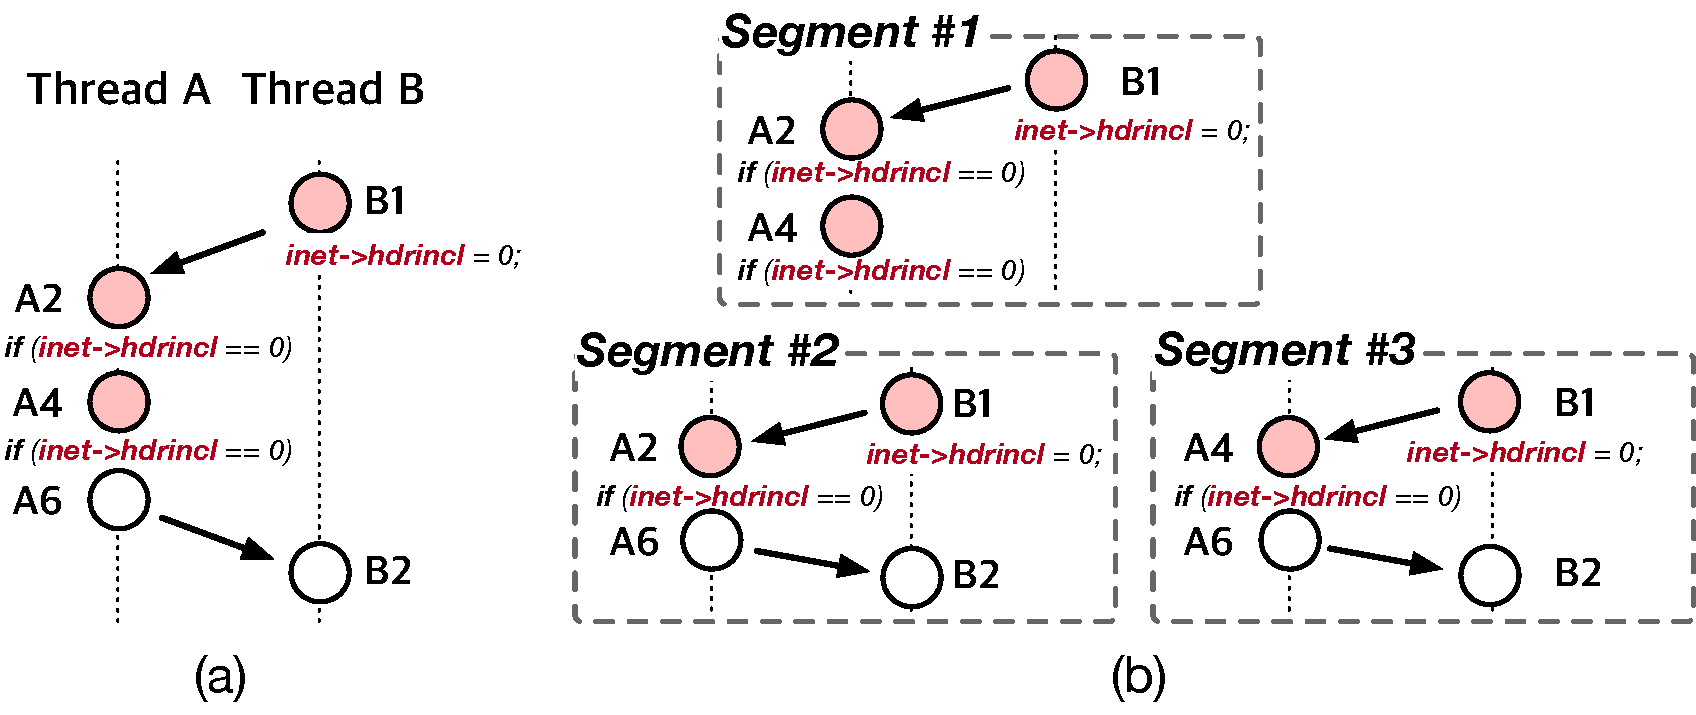
\includegraphics[width=0.99\linewidth]{fig/intuition.pdf}
  \caption{(a) A thread interleaving example of
    \autoref{fig:cve-2017-17712}, and (b) instruction segments
    contained in (a).  Note that we intentionally omit instructions
    that do not access globally-visible memory objects.}
  \label{fig:keyidea}
\end{figure}
%
\autoref{fig:keyidea} visualizes how we segmentize a thread
interleaving.
%
Let us assume we execute the two system calls in
\autoref{fig:cve-2017-17712} concurrently while monitoring memory
accesses annotated with timestamps.
%
We can then draw a totally-ordered instruction sequence of the thread
inteleaving as described in \autoref{fig:keyidea}-(a).



Segmentizing this thread interleaving is performed in two steps.
%
First, we pair up two instructions that access the same mermoy object.
%
In \autoref{fig:keyidea}-(a), there are three pairs of such
interleaved instructions such as
($\texttt{B1} \Rightarrow \texttt{A2}$) and
($\texttt{B1} \Rightarrow \texttt{A4}$) (accessing
\texttt{inet->hdrincl}), and ($\texttt{A6} \Rightarrow \texttt{B2}$)
(accessing \texttt{sk->owned}).
%
As we want to represent a combination of interleaving orders, the
second step is to further combine instruction pairs into an
interleaving segment.
%
Each interleaving segment is formed by combining two instruction pairs
so that interleaving segments contain at most four instructions.
%
For example, we combine two instruction pairs
($\texttt{B1} \Rightarrow \texttt{A2}$) and
($\texttt{B1} \Rightarrow \texttt{A4}$) to construct \texttt{Segment
  \#1} in which three instructions \texttt{B1}, \texttt{A2}, and
\texttt{A4} are included.
%
In accordance with timestamps annotated in these instructions, we can
arrange the instructions in \texttt{Segment \#1}.
%
Likewise, \texttt{Segment \#2} and \texttt{Segment \#3} are the result
of combining $\texttt{B1} \Rightarrow \texttt{A2}$ and
$\texttt{A6} \Rightarrow \texttt{B2}$, and
$\texttt{B1} \Rightarrow \texttt{A4}$ and
$\texttt{A6} \Rightarrow \texttt{B2}$ respectively.

%
% \autoref{fig:keyidea}-(a) represents the thread interleaving of the
% execution, where the uninitialized access bug does not manifest
% because \texttt{B1} is executed before \texttt{A4} (\ie,
% $(\texttt{A2} \Rightarrow \texttt{B1}) \wedge (\texttt{B1} \Rightarrow
% \texttt{A4})$ is not satisfied).
% %
% In order to track interleaving orders of a small number (\eg, four) of
% instructions, we decompose the thread interleaving into several
% interleaving segments as described in \autoref{fig:keyidea}-(b).
% %
% In these interleaving segments, \texttt{Segment \#1} contains three
% memory access operations (\ie, \texttt{A2}, \texttt{A4}, and
% \texttt{B1}), and describes interleaving orders such that \texttt{B1}
% is executed after \texttt{A2} and \texttt{A4}.
% %
% Similarly, \texttt{Segment \#2} and \texttt{Segment \#3} describes
% interleaving orders of four memory access operations, (\texttt{A2},
% \texttt{B1}, \texttt{B2}, \texttt{A6}) and (\texttt{A4}, \texttt{B1},
% \texttt{B2}, \texttt{A6}) respectively.
%

% With these interleaving segments, the fuzzer can be noticed that
% interleaving orders represented by these interelaving segments
% unlikley cause a concurrency bug.
% %
% Therefore, it is adequate for the fuzzer to search for unexplored
% interleaving segments (\eg, one that represents
% $(\texttt{A2} \Rightarrow \texttt{B1}) \wedge (\texttt{B1} \Rightarrow
% \texttt{A4})$) to maximize the chance of discovering concurrency bugs.


% %
% \dr{}
% It is worth noting that interleaving segments can be overlapped; in
% this example, \texttt{Segment \#1} and \texttt{Segment \#3} are
% overlapped over an interleaving order
% $\texttt{A4} \Rightarrow \texttt{B1}$.




\PP{Benefits of segmentizing thread interleaving}
%
Segmentizing thread interleaving provides two remarkable benefits to a
fuzzer as follows.



First, tracking interleaving segments is a befitting choice to
determine whether to further explore thread interleavings of a
multi-thread input.
%
% As mentioned above, most concurrency bugs manifest depending only on
% the execution order of four memory accesses.
%
Considering a concurrency bug manifests depending on a combination of
interleaving orders of at most four memory accesses (which is exactly
represented by an interleaving segment), if a fuzzer explores all
interleaving segments, it is unlikely that a fuzzer misses a
concurrency bugs.
%
Accordingly, \textit{interleaving segments can act as an
  interleaving coverage metric satisfying \textbf{Design goal 1}}.





\dr{}
Second, explored interleaving segments can be exploited to
systematically search thread interleavings to run in future
iterations.
%
Since each interleaving segment contains only a small number of memory
accesses, we can easily enumerate interleaving orders that these
memory accesses can produce.
%
Then, among enumerated interleaving orders, we can select ones that
unexplored before, and direct the fuzzer to search them.
%
In this way, \textit{we can satisfy \textbf{Design goal 2} by
  exploring meaningful thread interleavings at each iteration and
  minimizing redundant executions}.


% 
% \autoref{fig:hint} demonstrates how explored interleaving segments
% can be helpful for future iterations.
% %
% As illustrated in \autoref{fig:hint}, the fuzzer can derive
% \textit{unexplored} \texttt{Segment \#1*} by changing the execution
% order of \texttt{A4} and \texttt{B4} in \textit{explored}
% \texttt{Segment \#1}.
% %
% Since \texttt{Segment \#1*} satisfies
% $(\texttt{A2} \Rightarrow \texttt{B1}) \wedge (\texttt{B1} \Rightarrow
% \texttt{A4})$, the fuzzer can discover the uninitialized access bug if
% it executes thread interleaving containing \texttt{Segment \#1*}.
% %
% In addition, the fuzzer can explore multiple interleaving segments at
% a time.
% %
% Besides \texttt{Segment \#1*}, \texttt{Segment \#3*} can also be
% derived from \texttt{Segment \#3}.
% %
% Interestingly, \texttt{Segment \#1*} and \texttt{Segment \#3*} can be
% used to compose a new thread interleaving.
% %
% By executing a thread interleaving including the two derived
% interleaving segments, the fuzzer is able to quickly test a number of
% interleaving segments.
% %
% In this way, \textit{our proposed scheduler mechanism is designed to
%   quickly explore unexplored interleaving segments, and to satisfy
%   \textbf{R2}}.
% %
% \begin{figure}[t]
%   \centering
%   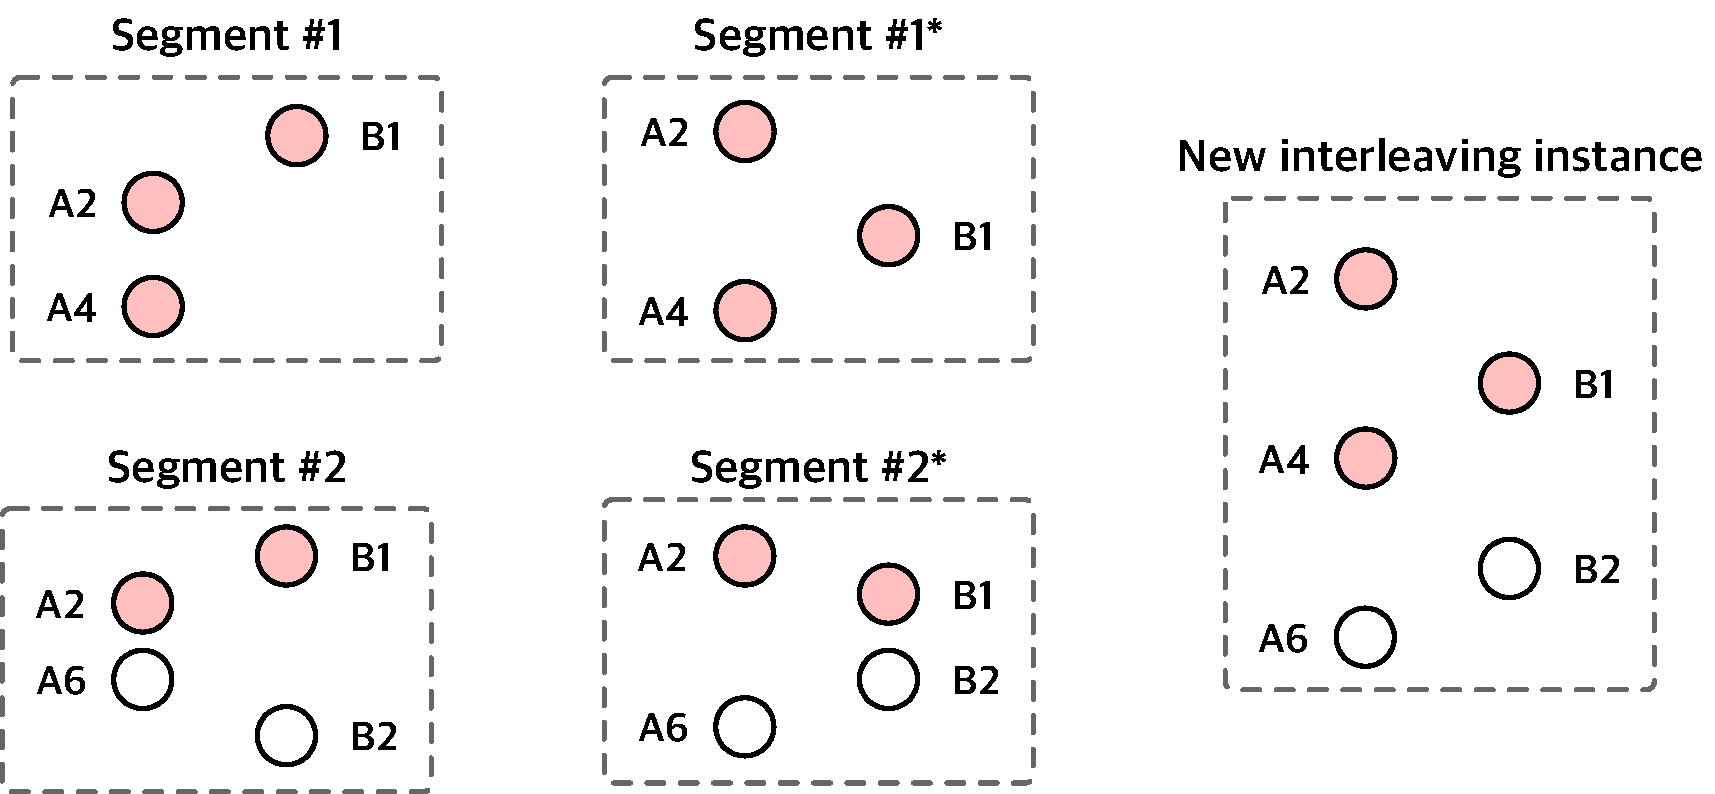
\includegraphics[width=0.9\linewidth]{fig/hint.pdf}
%   \caption{\texttt{Segment \#1} and \texttt{Segment \#3} are explored
%     interleaving segments in \autoref{fig:keyidea}.
%     %
%     From these two interleaving segments, our approach derives other
%     interleaving segments \texttt{Segment \#1*} and \texttt{\#3*}, and
%     schedules instructions to test the derived interleaving segments
%     at the same time.}
%   \label{fig:hint}
% \end{figure}
% %



\subsection{Interleaving Segment Coverage}
\label{ss:coverage}

\newcommand{\intcov}{interleaving segment coverage\xspace}
\newcommand{\Intcov}{Interleaving segment coverage\xspace}


Using a set of interleaving segments, we propose a novel interleaving coverage metric called \textit{\intcov}.
\Intcov is designed to track interleaving orders
within an interleaving segment and used for guiding a fuzzer to  
efficiently search possible instruction interleavings.
If \intcov of a given input is saturated, 
a fuzzer can confidently conclude that the input unlikely causes a concurrency bug and proceed to the next input.


\PP{Graph representation of interleaving segment}
% \PP{Graph representation of interleaved instructions}
As discussed, \intcov contains multiple interleaved instructions, 
so
% \intcov cannot be presented as a single instruction interleaving 
% (e.g., $I_x \rightarrow I_y$) used in the alias coverage used in KRace.
% Instead,
we represent each interleaving segment as a small directed acyclic
graph (DAG) called an interleaving segment graph (shortly, \textit{segment graph}), and \intcov is a collection of segment graphs.

In this graph, a vertex represents a memory-accessing instruction, 
and an edge represents an execution ordering between two memory-access instructions. 
Specifically, there are two types of edges, program-order edges and
interleaving-order edges.
%
A program-order edge indicates an execution order between two 
memory-accessing instruction in a single thread.
Whereas, an interleaving-order edge indicates the execution
order between two memory-access instructions that 1) access the same
shared data, 2) at least one of them is a write operation, and 3) are
executed by different threads.
\autoref{fig:interleavingsegmentgraph} illustrates how a segment
graph is derived from a interleaving segment, \texttt{Segment \#1}.
This segment graph contains a program-order edge from \texttt{A2} to
\texttt{A4} representing ``\texttt{A2} is executed before \texttt{A4}
in thread~A''.
Similarly, the segment graph contains two interleaving-order
edges, expressing interleaving orders of \texttt{B1} $\Rightarrow$ \texttt{A2}
and \texttt{B1} $\Rightarrow$ \texttt{A4}.
%It contains an interleaving-order edge from \texttt{A2} to
%\texttt{B1}, because 1) they access \texttt{inet->hdrincl}, 2)
%\texttt{B1} is a write operations, and 3) they are executed by
%different threads. Likewise, the segment graph also contains an
%interleaving-order edge from \texttt{A4} to \texttt{B1}.



\begin{figure}[t]
  \centering
  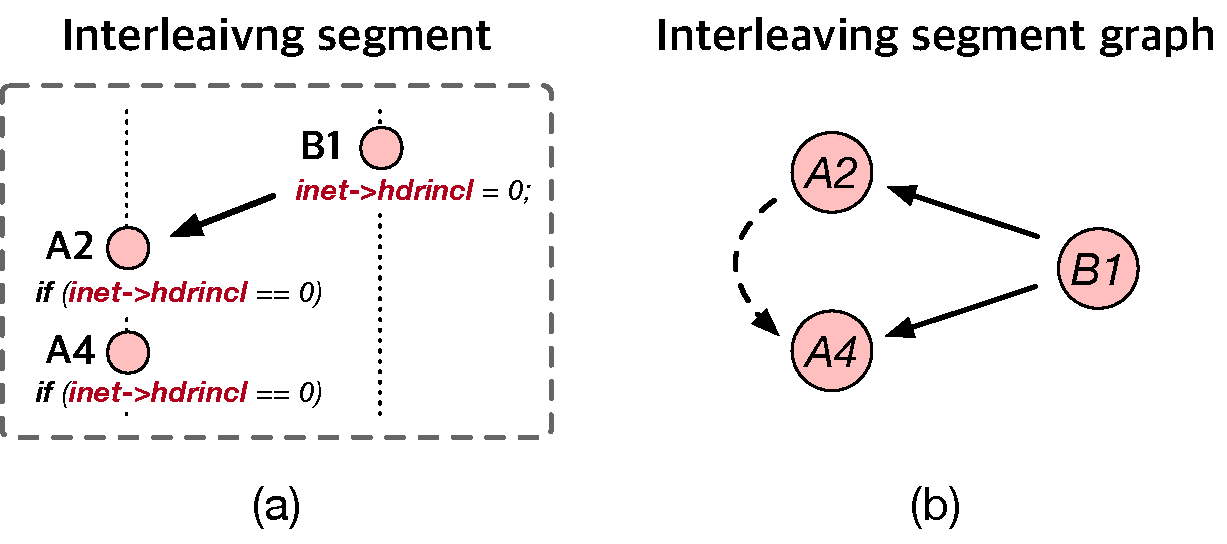
\includegraphics[width=0.8\linewidth]{fig/interleavingsegmentgraph.pdf}
  \caption{(a) \texttt{Segment \#1} from \autoref{fig:keyidea}, and
    (b) its segment graph. In (b), a dotted arrow represents a
    program-order edge, and solid arrows represent interleaving-order
    edges.}
  \label{fig:interleavingsegmentgraph}
\end{figure}

%It is worth noting that a segmentgraph has two properties. First, if
%a path exists from a vertex \texttt{X} to another vertex \texttt{Y}, a
%memory access operation corresponding to \texttt{X} is executed before
%a memory access operation corresponding to \texttt{Y}.
%%
%\dr{}
%This is because edges represent orderings that are a transitive
%relation.
%
%Second, \textit{all segment graph cannot contain a loop}.
%%
%If there is a loop exists, any vertex \texttt{Z} on the loop is
%executed before itself, which is contradictory.


%
% Let us represent a memory access operation $M$ as four tuples,
% $(tid, addr, op, timestamp)$ where $tid$ is the identity of a thread,
% $addr$ is the address of a memory location, $op$ is the type of the
% memory access operation (\ie, $store$ or $load$), and $timestamp$
% indicates the point of time when the memory access operation is taken.
% %
% $M(x)$ detnoes a field $x$ of $M$. For example, $M(tid)$ is a $tid$
% field of a memory access operation $M$.
% %
% Also let us suppose all memory access operations are totally
% ordered. \ie, there are no two memory access operations that have the
% same $timestamp$.

% For all pair of memory access operations $M_i$ and $M_j$, we define a
% scheduling constraint $SC$ as a tuple $(M_i, M_j)$ if
% $M_i(tid) \neq M_j(tid)$, $M_i(addr) = M_j(addr)$,
% $M_i(op) = store \vee M_j(op) = store$, and
% $M_i(timestamp) < M_j(timestamp)$.
% %
% Informally, $M_i$ and $M_j$ are conflicting memory acceess operations
% that are executed in other threads, and $M_i$ was taken place before
% $M_j$.
% %
% For two scheduling constraint $SC_1(M_{1i}, M_{1j})$ and
% $SC_2(M_{2i}, M_{2j})$, $SC_1 = SC_2$ if
% $(M_{1i} = M_{2i}) \wedge (M_{1j} = M_{2j})$.
% %
% Then, we define a scheduling constraint pair $SCPair = (SC_i, SC_j)$
% for two scheduling constraints if $i < j$, $SC_i \neq SC_j$.
% %
% Lastly, biconflict coverage of the concurrent job $BC\mbox{-}Cov$ is
% defined as a set of all scheduling constraint pairs,
% $\{SCPair_1, SCPair_2, ..., SCPair_n\}$, constructed from its memory
% access operation sequence.


\PP{Generating interleaving segment graph}
%
Let us assume executed memory accesses are represented in a list
($m_1$, $m_2$, ..., $m_k$). Without loss of generality, let us also
assume $m_i$ is executed before $m_j$ if $i<j$ (\ie, the list is
sorted in order of execution of memory accesses).
%
With this list of memory accesses, a fuzzer computes segment graphs in
two steps: generating a graph $g^*$ representing a whole thread
interleaving, and segmentizing the graph $g^*$ into subgraphs (\ie,
segment graphs).

Given a list of memory accesses, a fuzzer firstly generates vertices
$v_1$, $v_2$, ..., $v_k$ that correspond to executed memory accesses.
%
Then, for all $m_i, m_j$ such that $i<j$, a fuzzer generates a
directed edge $v_i \rightarrow v_j$ in two cases. A program-order edge
is generated if $m_i$ and $m_j$ are executed by the same thread.
%
Otherwise, an interleaving-order edge is generated if $m_i$ and $m_j$
are executed by different threads, they access the same memory object,
and one of them is a write operation.
%
After two types of edges are generated, some vertices are not
connected by any interleaving-order edge (in either direction), which
indicates that instructions corresponding to these vertices did not
access shared memory objects. And thus, these vertices and
corresponding instructions are not interesting when tracking thread
interleaving, and a fuzzer discards such vertices.
%
As a result, a fuzzer generates a set of vertices $V$ and a set of
edges $E$, where a graph $g = (V, E)$ representes a \textit{whole}
thread interleaving.


% \dr{I think formally describing how to construct interleaving graphs
%   is not a good idea.}
% %
% In order to formally explain how a fuzzer constructs interleaving
% graphs, let us assume executed memory accesses are represented in a
% list of four tuples, ($i_1$, $m_1$, $tid_i$, $ts_1$), ($i_2$, $m_2$,
% $tid_2$, $ts_2$), ..., ($i_k$, $m_k$, $tid_k$, $ts_k$), where $i$ is
% an instruction address, $m$ is an accessed memory object, $tid$ is a
% thread ID, and $t$ is a timestamp.
% %
% Without loss of generality, we also assume that the list is sorted
% according to timestamps (\ie, $ts_i < ts_j$ if $i < j$).


% Given a list of memory accesses, a fuzzer firstly generates vertices
% $v_1$, $v_2$, ..., $v_k$ for each memory accesses.
% %
% Then, for two vertices $v_{x}$ and $v_{y}$ such that $x < y$, a fuzzer
% generates directed edges $e = v_{x}$ $\rightarrow$ $v_{y}$ in two
% cases.
% %
% Otherwise, if $tid_{x} = tid_{y}$, then $e$ is generated as a
% program-order edge. If $m_{x}$ and $m_{y}$ are overlapped, then $e$ is
% generated as an interleaving-order edge.
% %
% As a result, a fuzzer constructs a set of vertices $V$ and a set of
% edges $E$, where a graph $g = (V, E)$ representes a \textit{whole}
% thread interleaving.




Afterwards, a fuzzer computes a set of subgraphs of $g^*$,
$G = \{g_1, g_2, ..., g_n\}$, where $g_i \in G$ has two
interleaving-order edges.
%
% For all $e_i, e_j \in E$ where
% $e_i = v_{x} \rightarrow v_{y}, e_j = v_{z} \rightarrow v_{w}, e_i
% \neq e_j$, a fuzzer constructs an interleaving graph
% $g_i = (V_i, E_i)$ such that $V_i$ is a set of
% $\{v_{x}, v_{y}, v_{z}, v_{w}\}$, and $E_i$ is a set of edges
% connecting vertices in $V_i$.
%
To this end, a fuzzer selects two interleaving-order edges
$e_x, e_y \in E$ such that $e_x \neq e_y$ (for example,
($\texttt{B1} \Rightarrow \texttt{A2}$) and
($\texttt{B1} \Rightarrow \texttt{A4}$) in
\autoref{fig:interleavingsegmentgraph}-(b)).
%
A fuzzer then forms a subgraph $g_i = (V_i, E_i)$ where $V_i$ is a set
of vertices that $e_x$ and $e_y$ connect (\ie, \texttt{B1},
\texttt{A2}, and \texttt{A4}), and $E_i$ is a set of edges connecting
vertices in $V_i$ (\ie, one program-order edge
($\texttt{A2} \Rightarrow \texttt{A4}$), and two interleaving-order
edges ($\texttt{B1} \Rightarrow \texttt{A2}$) and
($\texttt{B1} \Rightarrow \texttt{A4}$)).
%

Lastly, a fuzzer gathers interelaving graphs to form a set of
segment graphs $G = \{g_1, g_2, ..., g_n\}$, and uses $G$ to
track interleaving segment coverage and to search unexplored thread
interleavings.





\PP{Tracking interleaving segment coverage}
%
In practice, \intcov contains a large number of segment graphs,
which consumes a large amount of memory even though the size of graphs
is small.
%
To reduce memory consumption, we hash each segment graph, and
interleaving segment coverage tracks a hash table of segment graphs.
%
To this end, we adopt Merkel hashing~\cite{treehashing, treehashing2}.
%
The key property of Merkel hashing is reflecting directions of edges,
so that a fuzzer can distinguish different interleavings of the same
vertices.
%
% Due to space constraints, we
% present how $hash(g_i)$ can be used to distinguish different
% interleavings of the same vertices of
% \autoref{fig:interleavingmutation} in \autoref{s:appendix:hash}.



% \dr{I want to discuss about this part. I'm thinking taking this part
%   out to the appendix section:}
% %
% In particular, for all vertices $v$ in $V_i$, we first calculate a
% hash value of $v$, $hash(v)$, which reflects its out-going edges. With
% $o_1, ..., o_m$ that $v \rightarrow o_x \in E_i$,
% %
% %
% \\[1pt]
% \[
%   hash(v) = \mathcal{H}(v.label {++} o_1.label {++} ... {++}
%   o_m.label)
% \]
% \\[1pt]
% %
% where $\mathcal{H}$ denotes the
% non-cryptographic FNV hash function~\cite{fnv, fnv-go}, and ${++}$
% denotes the label-concatenation operation.
% %
% Then,
% %
% \\[1pt]
% \[
%   hash(g_i) = \underset{v \in V_i}{\oplus} hash(v)
% \]
% \\[1pt]
% %
% where $\oplus$ denotes the XOR operation. Due to space constraints, we
% present how $hash(g_i)$ can be used to distinguish different
% interleavings of the same vertices of
% \autoref{fig:interleavingmutation} in \autoref{s:appendix:hash}.





\PP{Utilizing interleaving segment coverage}
%
% \dr{I think it would be clearer not to mention alias coverage}
% %
% Compared to the alias coverage, \intcov and the form of interleaving graph
% express semantically richer information. \Intcov captures combinations 
% of multiple memory-accessing instructions as a unit of an interleaving segment, which allows a fuzzer to explore the large search space more quickly than using alias coverage, which uses a single instruction interleaving. Intuitively, across two different runs, \intcov can precisely tell 
% their differences in terms of at least two instruction interleavings, 
% but the alias coverage can tell at least one\yj{DR, it this claim OK to you?}.
% %
% \dr{no.. the search space of \intcov is larger than alias coverage. We
%   quickly explore the search space of \intcov because our search
%   strategy is clever, it is not because of the interleaving coverage.}
%
\Intcov and the form of segment graph express semantically rich
information; it captures combinations of multiple pairs of interleaved
instructions. At the same time, segment graphs are represented simply;
each segment graph contains only at most four instructions.

These two seemingly-conflicting characteristics of segment graphs
enables the systematic exploration of thread interleaving.
%
In other words, it is practically impossible to thoroughly explore all
thread interleavings of a given multi-thread input because of the
astronomical number of possible thread interleavings.
%
However, it is \textit{easily possible} to throughly explore
interleavings \textit{inside} interleaving segments due to their small
size. More importantly, exploring inside interleaving segments is
still enough to discover most concurrency bugs (as mentioned in
\autoref{ss:overview}).

Taking these advantages of \intcov, our interleaving search strategy
is \textit{not random} unlike previous approaches~\cite{krace, ski,
  pctalgorithm, muzz}, Rather, it is a systematic exploration
\textit{directed by explored interleaving coverage}.
%
\autoref{ss:scheduler} discusses our interleaving search strategy.


% \Intcov can guide the fuzzer to identify that there are possibly more
% useful instruction interleavings remain untested. So, the fuzzer
% spends more computing power to explore more interesting (unseen)
% instruction interleavings from \intcov. We emphasize that our
% searching strategy is \textit{not random} unlike previous
% approaches~\cite{krace, ski, pctalgorithm, muzz}.
% %
% We mutate a newly found interleaving graph to direct the fuzzer to
% systematically explore the search space of instruction interleavings
% while minimizing redundant and useless search
% trials.



\subsection{Coverage-directed Interleaving Search}
\label{ss:scheduler}
%
% One important role of segment graphs are to infer unexplored
% interleaving segments that the fuzzer will search for in future
% iterations.
% %
In this subsection, we explain how we utilize explored \intcov to
systematically explore thread interleavings.

\PP{Interleaving segment mutation}
%
The first step is to derive \textit{unexplored} interleaving graphs
from \textit{explored} interleaving graphs. We call this derivation
operation \textit{interleaving segment mutation} (shortly segment
mutation).
%
Suppose $G = \{g_1, g_2, ..., g_n \}$ is given for a thread
interleaving. Since $G$ is obtained after executing the thread
interleaving, all graphs in $G$ are \textit{explored}.
%
Then, a fuzzer mutates each $g_i \in G$ to drive other (and
unexplored) interleaving graphs.



\begin{figure}[t]
  \centering
  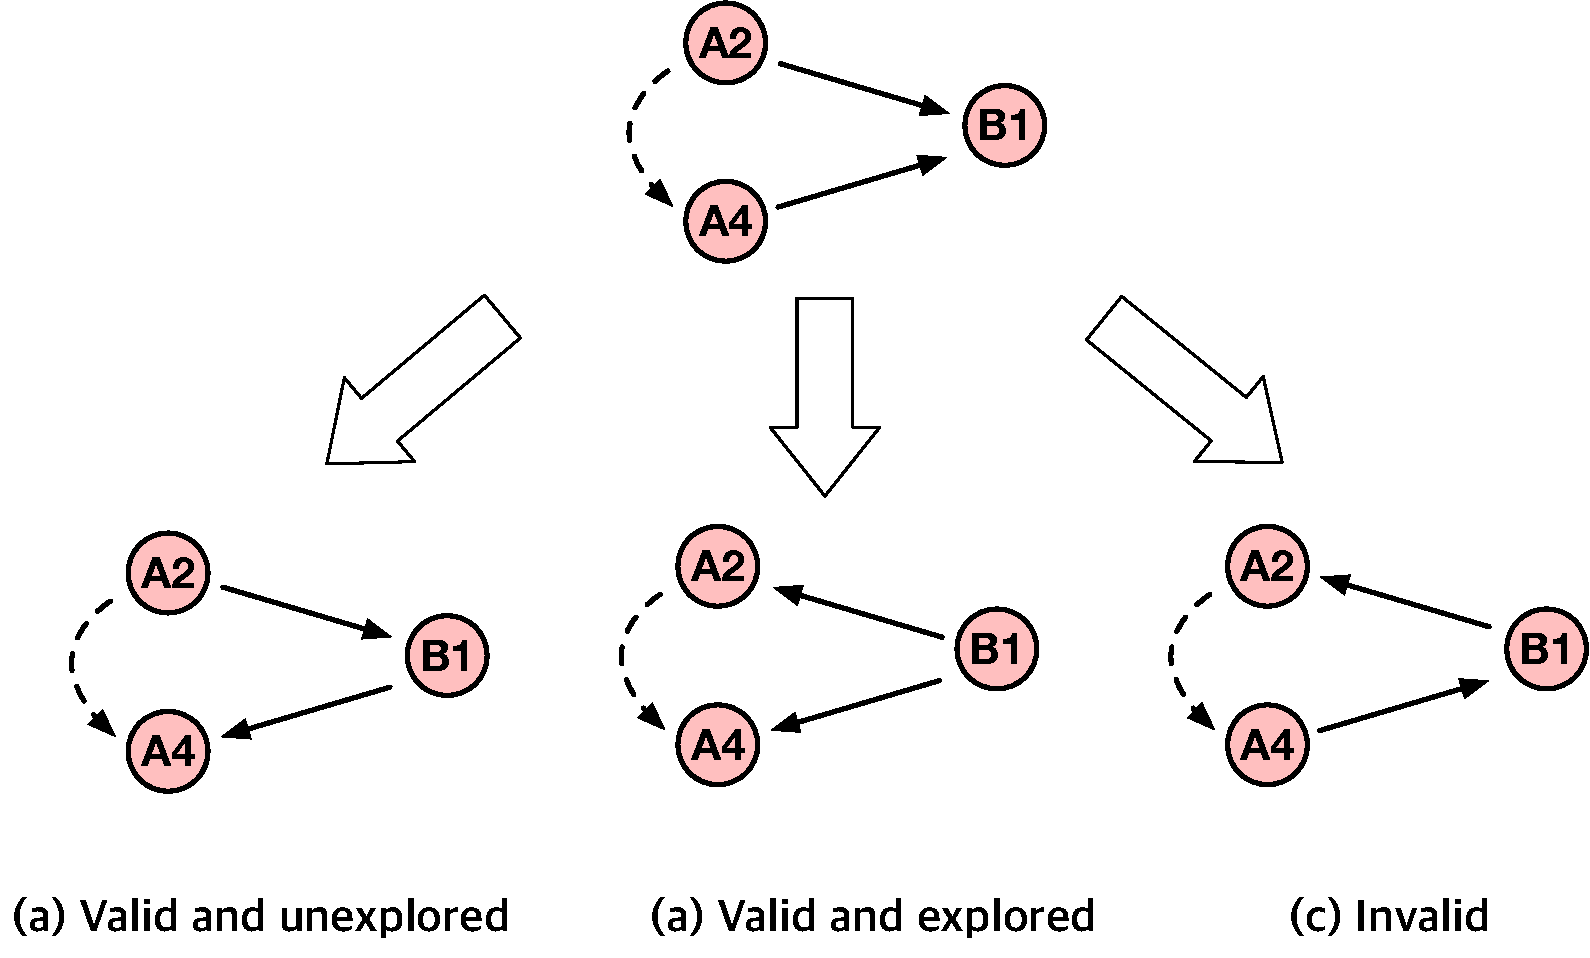
\includegraphics[width=0.7\linewidth]{fig/interleavingmutation.pdf}
  \caption{Example of interleaving segment mutation. In this example,
    (a) represents an interleaving segment graph of
    \autoref{fig:interleavingsegmentgraph} while (b) and (c) represent
    \textit{valid} mutations of (a). Whereas (d) is an
    \textit{invalid} mutation of (a) because it contains a loop.}
  \label{fig:interleavingmutation}
\end{figure}
%
\autoref{fig:interleavingmutation} illustrates how we mutate an
interleaving graph to derive other interleaving graphs.
%
We \textit{flip} interleaving-order edges (\ie, solid arrows) in an
interelaving graph described in
\autoref{fig:interleavingmutation}-(a), resulting in different
interleaving graphs.
%
The semantic behind ``\textit{flipping an interleaving-order edge}''
is simple; it changes the interleaving order of an instruction pair
that access the shared data.
%
For example, flipping ($\texttt{B1} \Rightarrow \texttt{A2}$) of
\autoref{fig:interleavingmutation}-(a) produces an interleaving graph
described in \autoref{fig:interleavingmutation}-(b), which describes a
different interleaving that \texttt{A2} is executed before
\texttt{B1}.
%
Likewise, we flip both of $\texttt{B1} \Rightarrow \texttt{A2}$ and
$\texttt{B1} \Rightarrow \texttt{A4}$ to generate an segment
graph of \autoref{fig:interleavingmutation}-(c).
%
Besides (a) and (b), however, flipping
$\texttt{B1} \Rightarrow \texttt{A4}$ of
\autoref{fig:interleavingmutation}-(a) generates an \textit{invalid}
segment graph that contains a loop as described in
\autoref{fig:interleavingmutation}-(d); a loop in an segment
graph indicates a contradiction on the execution order that any vertex
on the loop should be executed before itself.


\dr{TODO:}
In this way, a fuzzers mutates all $g_i \in G$, and aggregate all
mutated and unobserved interleaving segment graphs into $G_{mutated}$,
and uses it to search for a thread interleaving to run.

% Therefore, in this fugure, we can derive two \textit{unobserved}
% interleaving segment graphs.






\PP{Re-composing a thread interleaving}
%
One could naively test unexplored interleaving graphs in $G_{mutated}$
one-by-one.
%
However, it might require many executions because the size of
$G_{mutated}$ could be large.
%
Instead, we \textit{re-compose} a new thread interleaving from a
subset of $G_{mutated}$, and by running the re-composed thread
interleaving, we test multiple unexlored interleaving graphs at once.


\begin{figure}[t]
  \centering
  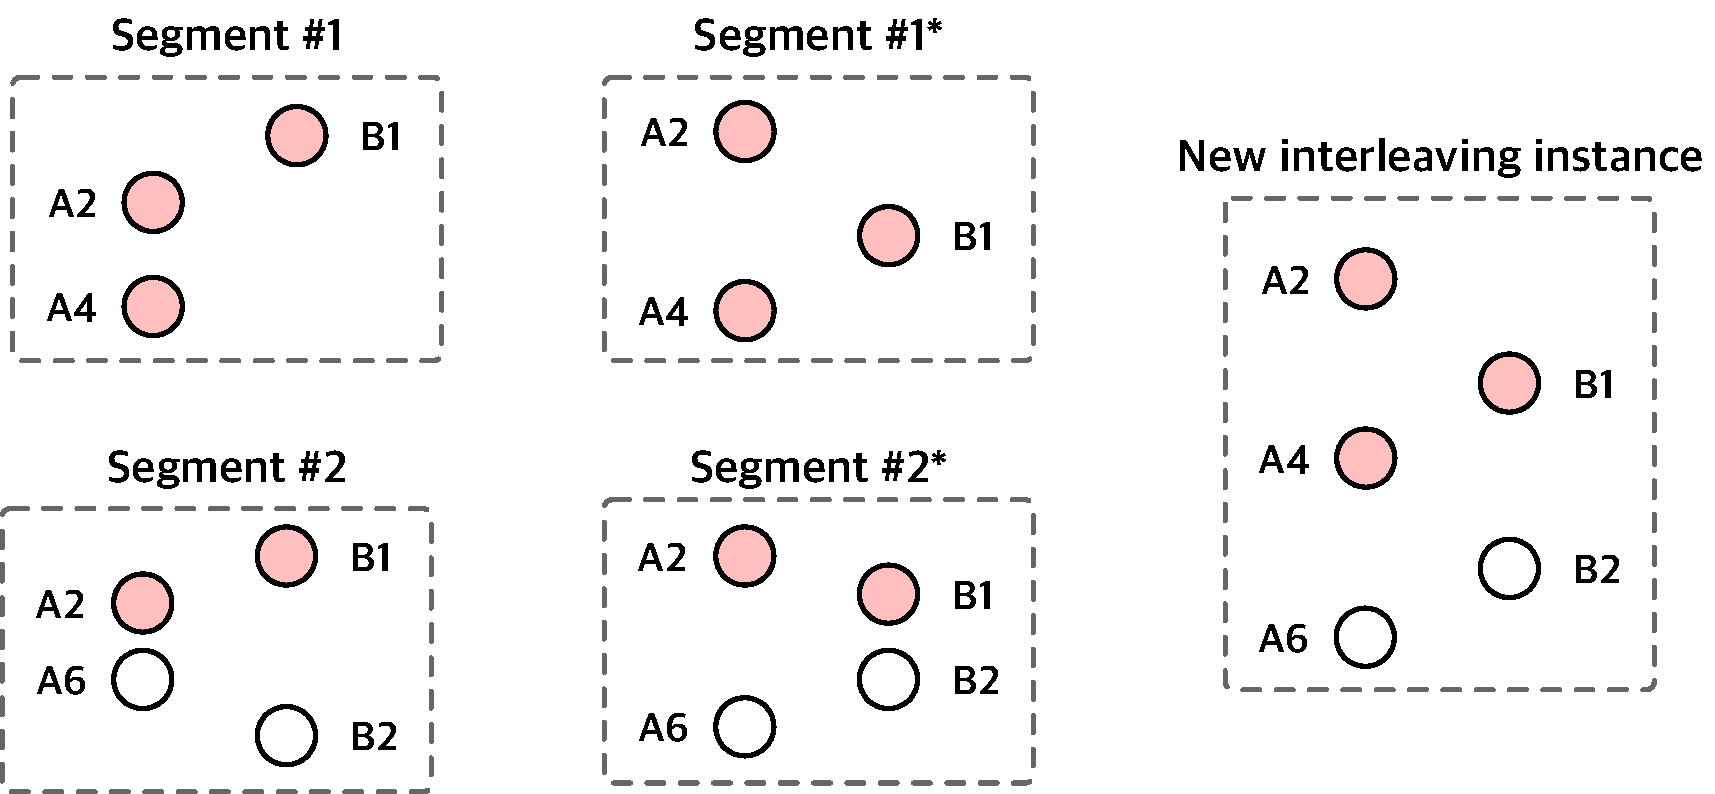
\includegraphics[width=0.8\linewidth]{fig/hint.pdf}
  \caption{}
  \label{fig:hint}
\end{figure}


\autoref{fig:hint} demonstrates an idea. Suppose we mutate explored
interleaving graphs in \autoref{fig:hint}-(a), and
\autoref{fig:hint}-(b) represents examples of mutated interleaving
segments, \texttt{Segment \#1*} and \texttt{Segment \#2*}.
%
We can then re-compose a new thread interleaving
\autoref{fig:hint}-(c) from \texttt{Segment \#1*} and \texttt{Segment
  \#2*}.


\dr{wip}
%
For each iteration, we select a subset of $G_{mutated}$ called
$G^{*}_{mutated}$, and search for a thread interleaving to explore all
unobserved interleaving segment graphs in $G^{*}_{mutated}$ at once.



It may require a heavy computation to identify the largest
contradiction-free subset of $G_{mutated}$.
%
Instead of finding an optimal solution, we choose to adopt a greedy
heuristic.
%
Specifically, we start with an empty set $\bar{G}$. Then, we iterate
over mutated segment graphs contained in given $G_{mutated}$, and
determine adding each segment graph into $\bar{G}$ forms a loop or
not. If it does not form a loop, we add the segment graph into
$\bar{G}$.
%
After iterating all mutated segment graphs in $G_{mutated}$, $\bar{G}$
does not contain a loop. The fuzzer then excludes selected segment
graphs from the set of all mutated segment graphs (\ie,
$G_{mutated} = S_{mutated} \setminus \bar{G}$), and generates
scheduling points to explore $\bar{G}$.









\PP{Generating scheduling points}
%
Once $G^{*}_{mutated}$ is given, scheduling points can be easily
generated by conducting a topological sort~\cite{topologicalsort}.
%
Since an imaginary interleaving graph is acyclic, a topological sort
always returns a sequence of vertices (\ie, instructions) that does
not violate a program order.
%
It is well known that the time complexity of a topological sort is
$O(V+E)$. Considering that the graph is sparse, $E$ is a small value
so the time complexity can be asymptotically considered as $O(V)$.
%
In this sequence, scheduling points are just instructions that the
preemption should happen; \ie, the next instruction is executed by a
different thread.




%%% Local Variables:
%%% mode: latex
%%% TeX-master: "p"
%%% End:
